\chapter{Partciles and The Large Hadron Collider}
\label{sec:particleslhc}

\section{The Standard Modell}
\label{sec:sm}

\section{particle decays and hadrons}
\label{sec:decays}

\section{The LHC and LHCb}
\label{sec:lhcandB}

\subsection{The LHC}
The Large Hadron Collider (LHC)\cite{lhcInfo} is the most powerfull particle-accelerator on planet earth. With a circumference of $26,7\si{\kilo\metre}$ it is also the longest ring accelerator and it lies between $45\si{\metre}$ and $170\si{\metre}$ below the surface near Geneva in Swizerland. The tunnel was constructed for the LEP experiment between 1984 and 1989 and is operated by the European Organization for Nuclear Research (CERN). The LHC can produce centre of mass energies of $\sqrt{s} = \SI{13}{\tera\electronvolt}$ in proton-proton collisions during Run 2. After the upgrade the LHC will collide particles with the centre of mass energy $\sqrt{s} = \SI{13}{\tera\electronvolt}$.
An image of the accelerators and the experiments is shown in fig. \ref{fig:CERN}\cite{facilityCERN}.

\begin{figure}
  \centering
  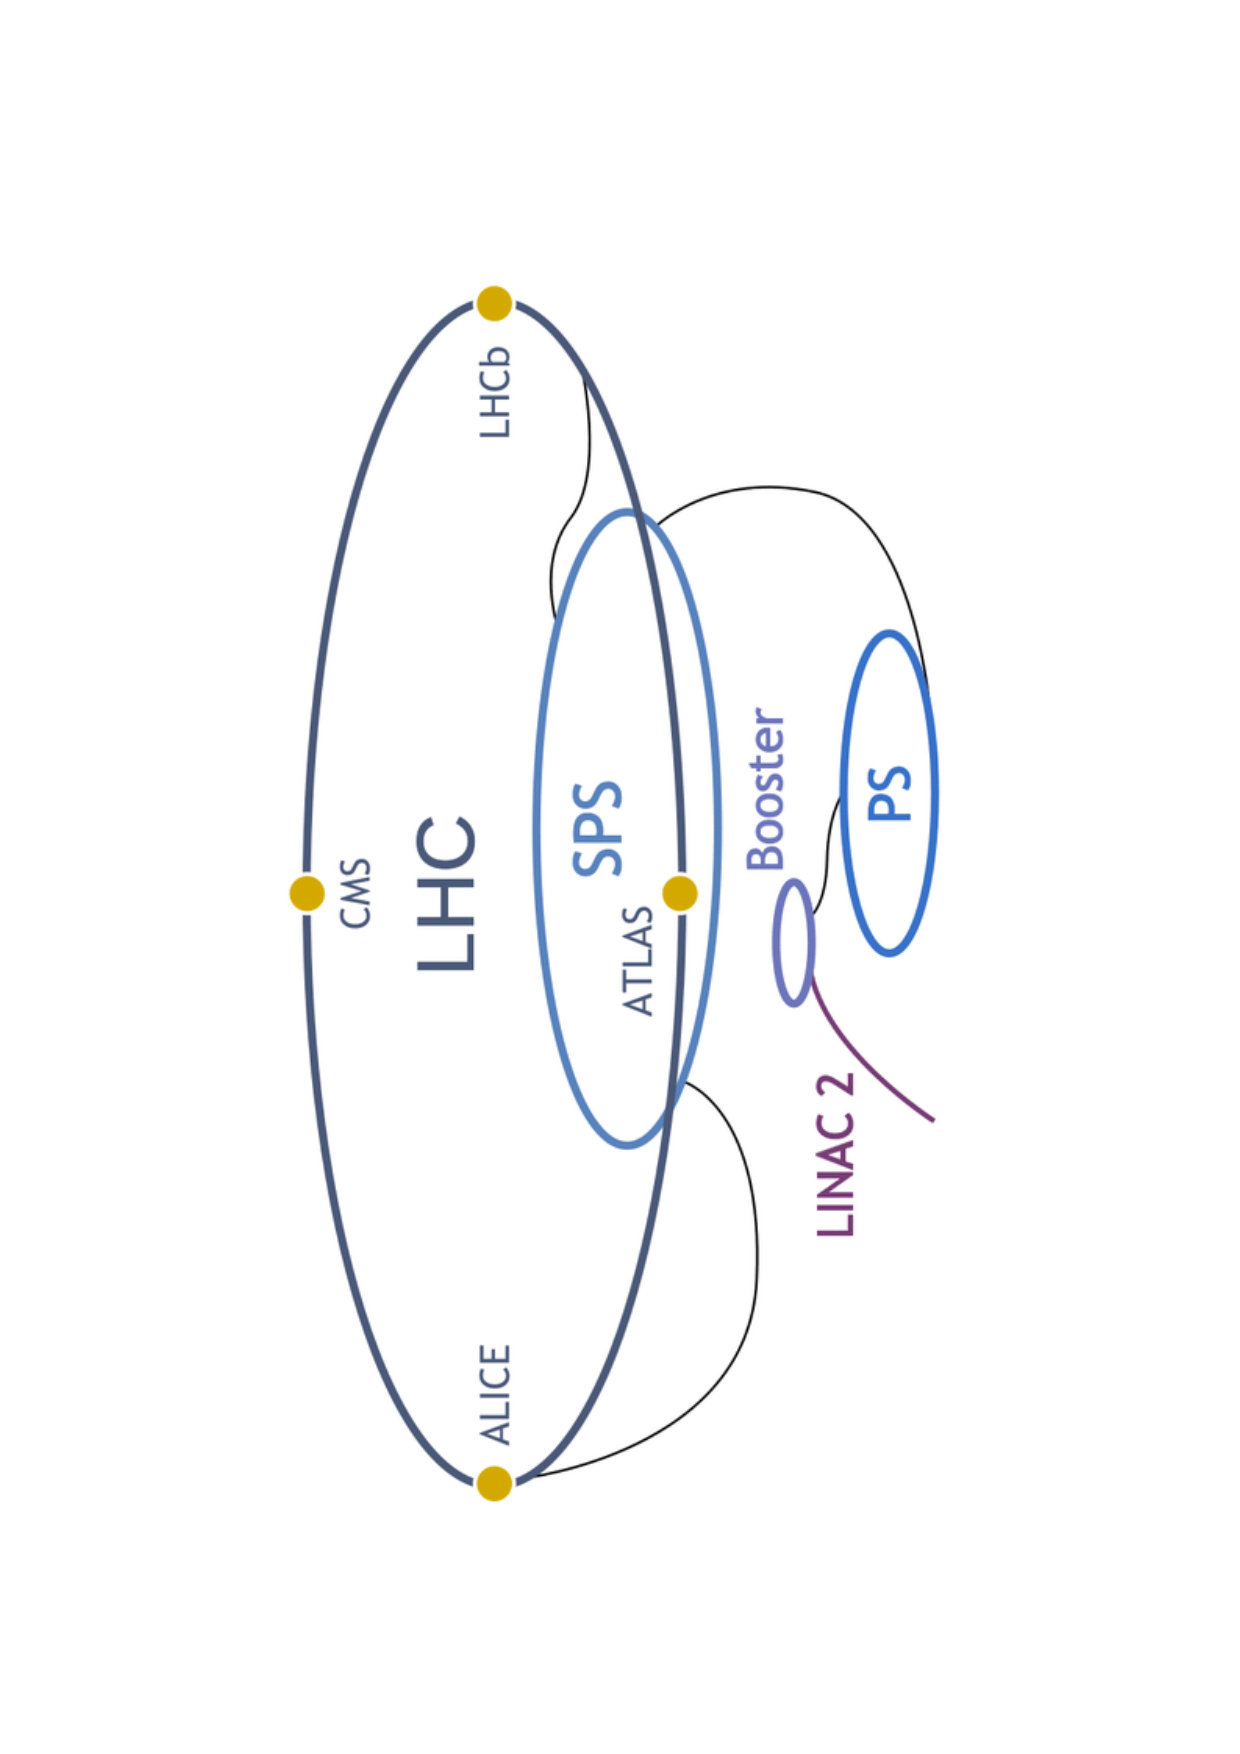
\includegraphics[angle=-90, origin=c, width=0.5\textwidth]{plots/CERN_layout.pdf}
  \caption{an overview of the LHC facilities.}
  \label{fig:CERN}
\end{figure}

By ionizing hydrogen gas, protonsare created and accelerated to $\SI{50}{\mega\electronvolt}$ by the linear accelerator (LINAC 2). Afterwards the beam is injected into the Proton Syncrotron and the Super Proton Synchrotron to a maximum of $\SI{450}{\giga\electronvolt}$ before the beam is brought into the LHC.
The beam containts several bunches with around $\num{1.15e11}$ and a bunch spacing of $\SI{25}{\nano\second}$, which is a collision rate of $\SI{40}{\mega\hertz}$.
The LHC houses four major experiments. ATLAS and CMS are classified as general purpose detectors with a detection range of close to $4\pi$. The interaction in these detectors is located in the very center so that tracks going in every direction can possibly be found. Searches for the Higgs Boson is just one of many physics aspects these detectors are build for.
The other two Experiments located at the LHC are ALICE and LHCb.
The ALICE experiment main studies the quark gluon plasma during the runs with lead ion collisions instead of protons.
In this thesis the Scintillating Fibre Tracker (SciFi Tracker) located at the LHCb will be focused at and discussed on the following chapters.

\subsection{The LHCb}

\begin{figure}
  \centering
  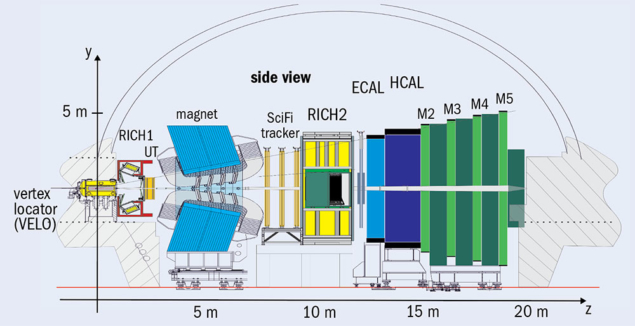
\includegraphics[width=0.5\textwidth]{plots/LHCb_facility.jpg}
  \caption{a sideview of the LHCb experiment.}
  \label{fig:LHCb}
\end{figure}

The LHCb experiment\cite{lhcbInfo} is a forward spectrometer covering $2 \less \eta \less 5$ in the pseudorapidity range. This experiments main physics goal is beauty quark physics and for high energies, b- and $\bar{b}$-hadrons are heavily produced in a tight forward direction\footnote{They are also produced in a tight backward direction but the experiment is only build for the forward cone.}. A sideview of the LHCb is shown in figure \ref{fig:LHCb}.
The LHCb consists of several smaller detector components namely the Vertex Locator (VELO) right on the intercation point, two Ring Imaging Cherenkov counter (RICH 1 and RICH 2), in front of the spectrometers lies the Trigger Tracker and behind them the SciFi Tracker which is the important part of this thesis. Further back a Scinitllator Pad Detector (SPD) and a Preshower (PS) are mounted followed by the electromagnetic calorimeter (ECAL) and the hadronic calorimeter (HCAL). In the very back, several muon chambers are mounted for every track that is yet to be determined.

In this section, a general overview about the requirements for the SciFi Tracker as well as the layout will be discribed based on the presentation in the \textit{technical design report}\cite{scifiInfo} of the upgrade.

The upstream and downstream trackers provide a good precision estimate of the momentum of charged particles so that mass resolution of decayed particles can be precisely measured. % this is a sentence i used from the TDR!
For particle identification the reconstructed trajectories of charegd particles are used as input for the RICH detectors.
The limiting factor for the momentum resolution is multiple scattering for tracks with a momentum lower than $\SI{80}{\giga\electronvolt\per\c}$. For tracks with a higher momentum the detector resolution is the limiting factor.

% why is the scifi there
The SciFi Tracker replaced the inner Tracker (IT) and the outer Tracker (OT) and is located in the same place as the downstream trackers that were previously installed.

% data and facts
The instantaneous luminosity after the upgrade is expected to be $\SIrange{1}{2e33}{\per\centi\metre\squared\per\second}$. The bunch spacing will be $\SI{25}{\nano\second}$ and the number of proton-proton interactions per bunch crossing will be $\nu = 3.8$ during the ramp-up phase of the LHC and $\nu = 7.6$ "during the active phase." (how can i write this differently?)

% layout
\subsection{Layout of the Detector}
The SciFi Tracker consists of three (T-)stations T1, T2 and T3 with each having four Layers ($X1, U, V, X2$). The orientation of these planes with respect to the vertical axis are ($\SI{0}{\degree}, \SI{+5}{\degree}, \SI{-5}{\degree}, \SI{0}{\degree}$).
The tilted layers are called stereo layers and serve the purpose of 3D hit localization.
Each layer consists of 8 fibremats
A right-handed coordinate system is used with positive $z$ pointing away from the interaction point following the beam direction. positive $y$ points upwards, towards the surface and positive $x$ and negative $x$ are defined as A-Side and C-Side\cite{scifiInfo}.

% \begin{enumerate}
%   \item layout
%   \item how does it work?
%   \item what else?
% \end{enumerate}

\section{The LHC data cycle}
\label{sec:datacycle}

(not sure if that's a good name, but like, an explanation of how electrical information is turned into hits and then tracks, and also when alignment runs in the system of data taking)
